\begin{enumerate}
\item Represent the following situation mathematically:
\begin{enumerate}[label=(\roman*)]
\item John and Jevanti together have $45$ marbles. Both of them lost $5$ marbles each, and the product of the number of marbles they now have is $124$. We would like to find out how many marbles they had to start with.
\item A cottage industry produces a certain number of toys a day. The cost of production of each toy (in Rupees) was found to be $55$ minus the number of toys produced in a day. On a particular day, the total cost of production was \rupee~750. We woud like to find out the number of toys produced on that day.
\end{enumerate}
\item Check whether the following are quadratic equations:
\begin{enumerate}[label=(\roman*)]
\item $(x-2)^2+1=2x-3$
\item $x(x+1)+8 = (x+2) (x-2)$
\item $x(2x+3) = X^2+1$
\item $(x+2)^3 = x^3-4$
\end{enumerate}
\item Find the roots of the equation $2x^2 -5x+3 = 0$  by factorisation.
\item Find the roots of the quadratic equation $6x^2 -x-2 = 0$.
\item Find the roots of the quadratic equation $3x^2 -2\sqrt6x+2 = 0$
\item Find the dimensions of the prayer hall discussed in Section $4.1$. A charity trust decides to build a prayer hall having a carpet area of 300 square metres with its length one metre more than twice its breath. What should be the length and breadth of the hall?
\item Solve the equation given in Example $3$ by the method of completing the square.
\item Find the roots of the equation $5x^2-6x-2 = 0$ by the method of completing the square.
\item Find the roots of $4x^2+3x+5 = 0$ by the method of completing the square.
\item Solve Q.2(i) of exercise $4.1$ by using the quadratic formula.
\begin{enumerate}[label=(\roman*)]
\item The area of a rectangle plot is $528 m^2$. The length of the plot (in metres) is one more than twice itsbreadth. We need to find the length and breadth of the plot.
\end{enumerate}
\item Find two consecutive odd positive integers, sum of whose squares is $290$.
\item A rectangular park is to be designed whose breadth is $3$ m less than its length. Its are is to be $4$ square metres than the area of a park that has already been made in the shape of a isoceles triangle with its base as  the breadth of the rectangular park and of altitude $12$ m (see \figref{fig:4.3}). Find its length and breadth.
\begin{figure}[h]
\centering
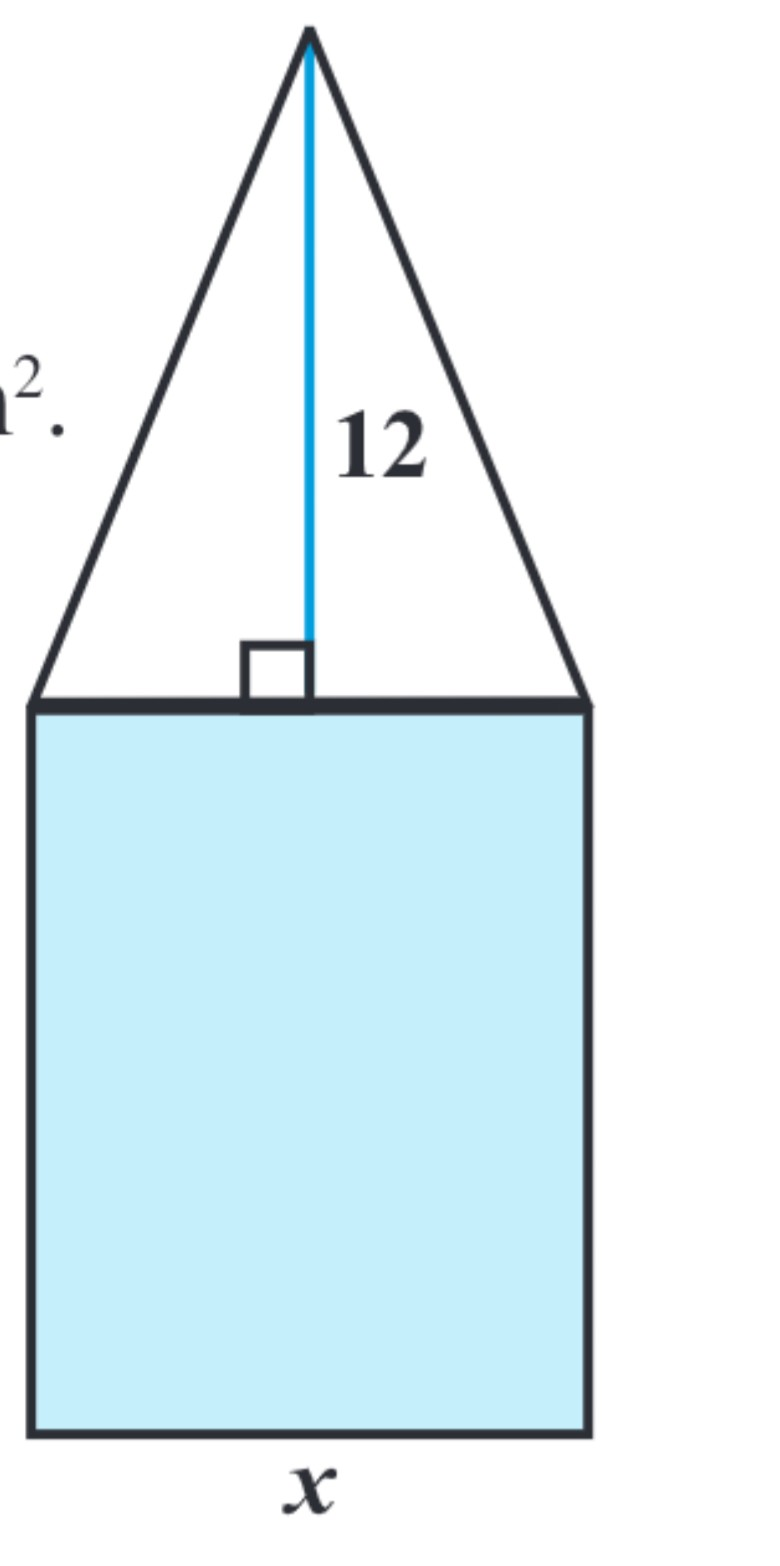
\includegraphics[width=\columnwidth]{chapters/10/figs/4.3.png}
\caption{4.3}
  \label{fig:4.3}
\end{figure}
\item Find the roots of the following quadratic equations, if they exist, using the quadratic formula.
\begin{enumerate}[label=(\roman*)]
\item $3x^2-5x+2 = 0$
\item $x^2+4x+5 = 0$
\item $2x^2-2\sqrt 2x+1 = 0$
\end{enumerate}
\item Find the roots of the following equations:
\begin{enumerate}[label=(\roman*)]
\item $x+\frac{1}{x} = 3,x\neq0$
\item $\frac{1}{x}-\frac{1}{x-2} = 3, x\neq 0,2$
\end{enumerate}
\item A motor boat whose speed is $18$ km/h in still water takes $1$ hour more to go $24$ km upstream than to return downstream to the same spot. Find the speed of the stream.
\item Find the discriminant of the quadratic equation $2x^2-4x+3 = 0$, and hence find the nature of its roots.
\item A pole has to be erected at a point on the boundary of a circular park of diameter $1.3$ metres in such a way that the difference of its distances from two diametrically opposite fixed gates A and B on the boundary is $7$ metres. Is it possible to do so? If yes, at what distances from the two gatees should the pole be erected ?
\item Find the discriminant of the equation $3x^2-2x+\frac{1}{3} = 0$ and hence find the nature of its roots. Find them, if they are real.
\end{enumerate}
